% !TeX encoding = UTF-8
% !TeX spellcheck = es_AR
% arara: pdflatex
% arara: pdflatex
% arara: pdflatex
% arara: clean: {files: [01_informatica_basica.aux, 01_informatica_basica.out, 01_informatica_basica.log]}
% arara: clean: {files: [01_informatica_basica.fdb_latexmk, 01_informatica_basica.fls, 01_informatica_basica.vrb, 01_informatica_basica.synctex.gz]}

%% Add the word "answers" to document class parameters in order to print the solutions.
\documentclass[12pt, addpoints]{../../common/epyl_exam_template}

\title{Práctica 1.1 - Informática Básica}
\date{2018.1}

\begin{document}
\makeexamheader
\makeexamtitle
\examrule
\begin{questions}
  \question
  Analice el anuncio del smartphone que se presenta a continuación y responda:
  \\~\\
  \centerline{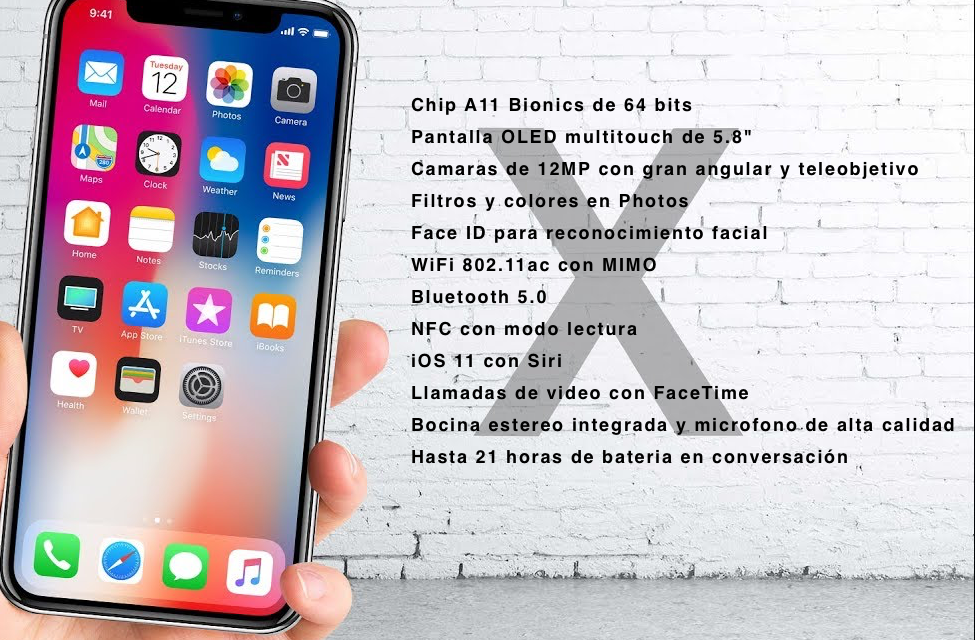
\includegraphics[scale=0.4]{img/iphone_x_specs.png}}
  \begin{parts}
    \part
      ¿Qué elementos de la publicidad aluden al hardware del equipo?
      \begin{solution}
        Chip A11 Bionics de 64 bits
        Pantalla OLED multitouch de 5.8"
        Cámaras de 12MP con gran angular y teleobjetivo
        WiFi 802.11ac con MIMO
        Bluetooth 5.0
        NFC con modo lectura
        Bocina estéreo integrada y micrófono de alta calidad
        Hasta 21hs de batería en conversación
      \end{solution}
    \part
      ¿Qué elementos aluden al software del equipo?
      \begin{solution}
        Filtros y colores en Photos
        FaceID para reconocimiento facial
        iOS 11 con Siri
        Llamadas de video con FaceTime
      \end{solution}
  \end{parts}
  \question
  Considere los siguientes nombres completos de archivos y determine de
  qué tipo de archivo se trata (imagen, audio, texto, programa, etc.).
  Puede buscar la extensión en internet para tener más información sobre
  la misma en caso de que la desconozca.
  \begin{parts}
    \begin{minipage}{0.5\textwidth}
      \part acdc.jpg \begin{solution} Imagen JPG \end{solution}
      \part ringtone.wav \begin{solution} Audio sin comprimir \end{solution}
      \part subtitles\_tbbt\_s01e04.zip \begin{solution} Archivo comprimido con ZIP \end{solution}
      \part configuration.xml \begin{solution} Documento de texto XML \end{solution}
      \part informacion.txt \begin{solution} Documento de texto plano \end{solution}
      \part runtime.py \begin{solution} Documento de texto con código Python \end{solution}
    \end{minipage}
    \begin{minipage}{0.5\textwidth}
      \part day\_of\_the\_tentacle.exe \begin{solution} Archivo ejecutable de Windows \end{solution}
      \part contabilidad.xls \begin{solution} Hoja de cálculo de Excel \end{solution}
      \part investors\_showcase.ppt \begin{solution} Presentación de PowerPoint \end{solution}
      \part cv.docx \begin{solution} Documento de texto de Word \end{solution}
      \part run.ini \begin{solution} Archivo de texto de configuración \end{solution}
      \part startup.sh \begin{solution} Archivo de texto con código Bash \end{solution}
    \end{minipage}
  \end{parts}
  \question
  Dados los siguientes árboles de carpetas para un sistema Windows, y Linux.
  \\~\\
  \begin{minipage}{0.5\textwidth}
    \centerline{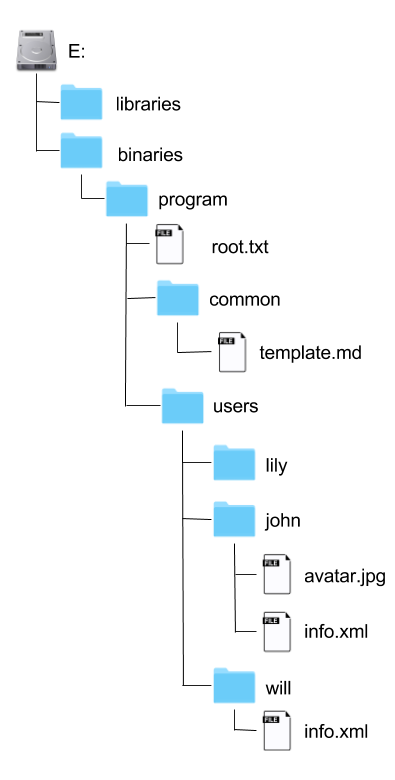
\includegraphics[scale=0.4]{img/folders_windows.png}}
  \end{minipage}
  \begin{minipage}{0.5\textwidth}
    \centerline{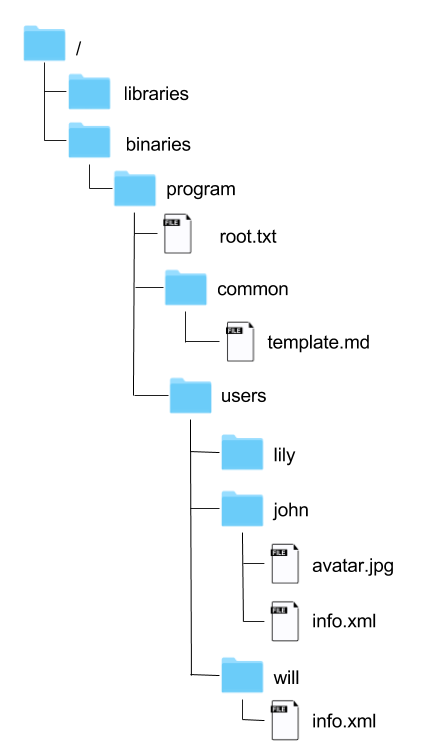
\includegraphics[scale=0.4]{img/folders_unix.png}}
  \end{minipage}
  \begin{parts}
    \part Indique que carpetas están vacías.
      \begin{solution} libraries, lily \end{solution}
    \part Indique la ruta al directorio raíz del sistema.
      \begin{solution} Windows: E:, Linux: / \end{solution}
    \part Indique la ruta absoluta para cada archivo que se muestra en el árbol.
      \begin{solution}
        Windows:
        \begin{itemize}
          \item \url{E:\\binaries\\program\\root.txt}
          \item \url{E:\\binaries\\program\\common\\template.md}
          \item \url{E:\\binaries\\program\\users\\john\\avatar.jpg}
          \item \url{E:\\binaries\\program\\users\\john\\info.xml}
          \item \url{E:\\binaries\\program\\users\\will\\info.xml}
        \end{itemize}
        Linux:
        \begin{itemize}
          \item \url{/binaries/program/root.txt}
          \item \url{/binaries/program/common/template.md}
          \item \url{/binaries/program/users/john/avatar.jpg}
          \item \url{/binaries/program/users/john/info.xml}
          \item \url{/binaries/program/users/will/info.xml}
        \end{itemize}
      \end{solution}
    \part Indique la ruta relativa al archivo ``root.txt'' para cada archivo.
    \begin{solution}
      Windows:
      \begin{itemize}
        \item \url{common\\template.md}
        \item \url{users\\john\\avatar.jpg}
        \item \url{users\\john\\info.xml}
        \item \url{users\\will\\info.xml}
      \end{itemize}
      Linux:
      \begin{itemize}
        \item \url{common/template.md}
        \item \url{users/john/avatar.jpg}
        \item \url{users/john/info.xml}
        \item \url{users/will/info.xml}
      \end{itemize}
    \end{solution}
    \part Indique la ruta relativa al archivo ``template.md'' para cada uno de los archivos de la carpeta ``users''.
    \begin{solution}
      Windows:
      \begin{itemize}
        \item \url{..\\users\\john\\avatar.jpg}
        \item \url{..\\users\\john\\info.xml}
        \item \url{..\\users\\will\\info.xml}
      \end{itemize}
      Linux:
      \begin{itemize}
        \item \url{../users/john/avatar.jpg}
        \item \url{../users/john/info.xml}
        \item \url{../users/will/info.xml}
      \end{itemize}
    \end{solution}
  \end{parts}
\end{questions}
\end{document}
